\documentclass[english]{VUMIFPSbakalaurinis}

% Used packages
\usepackage{float}
\usepackage{wrapfig2}
\usepackage{hyperref}
\usepackage{algorithmicx}
\usepackage{algorithm}
\usepackage{algpseudocode}
\usepackage{amsfonts}
\usepackage{amsmath}
\usepackage{bm}
\usepackage{caption}
\usepackage{color}
\usepackage{graphicx}
\usepackage{listings}
\usepackage{subcaption}
\usepackage{biblatex}

% Title page
% Titulinio aprašas
\university{Vilnius university}
\faculty{Faculty of mathematics and informatics}
\department{Bachelor's degree programme in software engineering}
\papertype{Bachelor's thesis}
\title{Gyventojų skaičiaus prognozavimas iš palydovinių vaizdų}
\titleineng{Population forecasting from satellite images}
\author{Lukas Brasiūnas}
\supervisor{assoc. prof. Valentas Gružauskas}
\reviewer{doc. dr. Vardauskas Pavardauskas}
\date{Vilnius – \the\year}

\bibliography{references}

\begin{document}
\maketitle

% Summaries
\begin{lithuanian}
\sectionnonumnocontent{Santrauka}
Glaustai aprašomas darbo turinys: pristatoma nagrinėta problema ir padarytos
išvados. Santraukos apimtis ne didesnė nei 0,5 puslapio. Santraukų gale
nurodomi darbo raktiniai žodžiai. Automatiškai naudojamos lietuviškos kabutės: \enquote{tekstas}.

% Nurodomi iki 5 svarbiausių temos raktinių žodžių (terminų).
% Vienas terminas gali susidėti iš kelių žodžių.
\raktiniaizodziai{raktinis žodis 1, raktinis žodis 2, raktinis žodis 3, raktinis žodis 4, raktinis žodis 5}
\end{lithuanian}

\begin{english}
\sectionnonumnocontent{Summary}
Santrauka anglų kalba. Santraukos apimtis ne didesnė nei 0,5 puslapio. Automatiškai naudojamos angliškos kabutės: \enquote{tekstas}.

\keywords{keyword 1, keyword 2, keyword 3, keyword 4, keyword 5}
\end{english}

% Table of contents
\tableofcontents

% Introduction
\sectionnonum{Introduction}

The industrial revolution, which began in the late 18th century and continued into the 19th, had a profound impact on population growth, laying the foundation for the demographic explosion that the world knows today. It brought some important industrial changes including advancements in agriculture, public health, transportation, communication that dramatically altered living conditions without which humans would not be as successful as they are today. This major humanity milestone has advanced humans but as a consequence introduced some important problems that are being faced right now.

Today 4.4 billion people live in cities which is expected to increase, with the urban population more than doubling its current size by 2050, which would translate in 7 out of 10 people living in the cities \cite{WrldBnkUrbanDevelopment}. This shows the importance of city planning and world resource allocation and budgeting in order for humanity to be prosperous today and in the future. This means that country governments and other institutions need to conduct population forecasting censuses in order to make important decisions when it comes to existing and new city planning. Current methods of taking population censuses are outdated, take a large amount of time and are conducted quite rarely - at least once every 10 years in developed countries. Traditional current census conducting methods include registration of all individuals and their details using questionnaires during online and real-life campaigns which last from a few days to couple of weeks or even months. Another popular approach is conducted using population registers and other administrative sources without the need of collecting population information via questionnaires \cite{CensusApproachesAndMethods}. This shows that a need of new, faster, cheaper and more accurate, population forecasting methods analysis and implementation is essential.

This work includes detailed analysis of literature in order to understand current population forecasting methods in depth, their pitfalls and strengths, when it comes to a rapidly changing world and it's urban environment. The thesis describes both currently used population census conducting methods in detail and analyses an alternative method using data that is already widely available on the internet to analyse its' potential when it comes to population forecasting - using deep learning and neural network models.

This thesis analyses and compares the speed, accuracy and resources needed for a couple of chosen neural network models (\textbf{TO-DO: NAME THE CHOSEN MODELS HERE}) when it comes to forecasting population using satellite images. The analysis and comparison will be done using a custom dataset consisting of coloured orthographic maps and population statistics in a specific area.

This work will grant a conclusion as to which neural network model is best fit for this type of population forecasting using satellite images. The study aims to identify which model is best fit when it comes to population census based on different evaluation criteria such as speed, accuracy, loss and resources needed to train the model. To achieve the desired goal, tasks defined further need to be completed:
\begin{enumerate}
    \item Task 1 \textbf{TO-DO: Write the tasks that need to be completed in order to achieve the desired goal.}
    \item Task 2
    \item Task 3
    \item Task 4
    \item Task 5
\end{enumerate}

% Overviews
\section{Overview of population forecasting methods}

Population forecasting is the practice of predicting future population sizes and structures based on current demographic data, trends, and assumptions regarding factors like fertility rates, mortality rates, and migration flows. These forecasts are crucial for policymakers, urban planners, and organizations in planning for future needs in healthcare, education, infrastructure, housing, and employment. By understanding potential population shifts, governments can allocate resources effectively and prepare for aging populations, urban growth, or potential labor shortages.

An essential tool that underpins population forecasting is the population census. A census is a systematic effort to collect detailed information about every individual within a country or region, including data on age, sex, race, education, employment, and living conditions. Conducted typically every 10 years, censuses provide a comprehensive snapshot of a population at a specific moment in time. This data is not only crucial for immediate decision-making but also serves as the foundation for future demographic analysis and projections. Without accurate and timely census data, population forecasts would lack a reliable baseline, making predictions about future demographic changes significantly less accurate.

Censuses have a long history, dating back to ancient civilizations like Egypt and Rome, where they were used primarily for taxation and military conscription purposes. The modern concept of the census, however, began in Sweden in 1749 and spread to other European countries in the centuries that followed \cite{BirthOfModernCensusInSweden}. In the United States, the first national census was conducted in 1790 and has been carried out every decade since, even helping other countries around the world conduct their own censuses \cite{UsaHelpingOthersWithCensuses}. Over time, census methods have evolved from basic headcounts to more sophisticated surveys, incorporating data collection techniques that include digital tools, administrative records, and statistical sampling.

Censuses are typically conducted through a combination of self-reporting by households, in-person interviews, and administrative record analysis. The process generally starts with extensive planning and public outreach to ensure high participation rates. Census workers are employed to visit households and collect data either through interviews or by delivering and retrieving census forms. In many countries, individuals are encouraged to complete the census forms online or via mail, offering a more efficient and cost-effective method of data collection. The forms usually cover essential demographic details such as age, sex, household size, educational attainment, occupation, and housing characteristics. Modern censuses are increasingly utilizing digital tools and new technologies to streamline the collection and processing of data, helping governments to obtain more accurate and timely population information \cite{CensusPrinciplesAndRecommendations}.

The most recent 2020 round of population censuses was a global effort where many countries conducted their censuses, despite facing significant challenges due to the COVID-19 pandemic \cite{Codid19ImplicationsOnCensusConduct}. The pandemic disrupted traditional census operations, leading to delays, changes in methodology, and increased reliance on digital and administrative data collection methods. Some countries moved more census processes online to reduce in-person contact, while some, postponed their census altogether. The 2020 round highlighted the growing importance of digital tools, remote data collection, and administrative records in ensuring accurate population counts during unforeseen circumstances.

\begin{figure}[H]
    \centering
    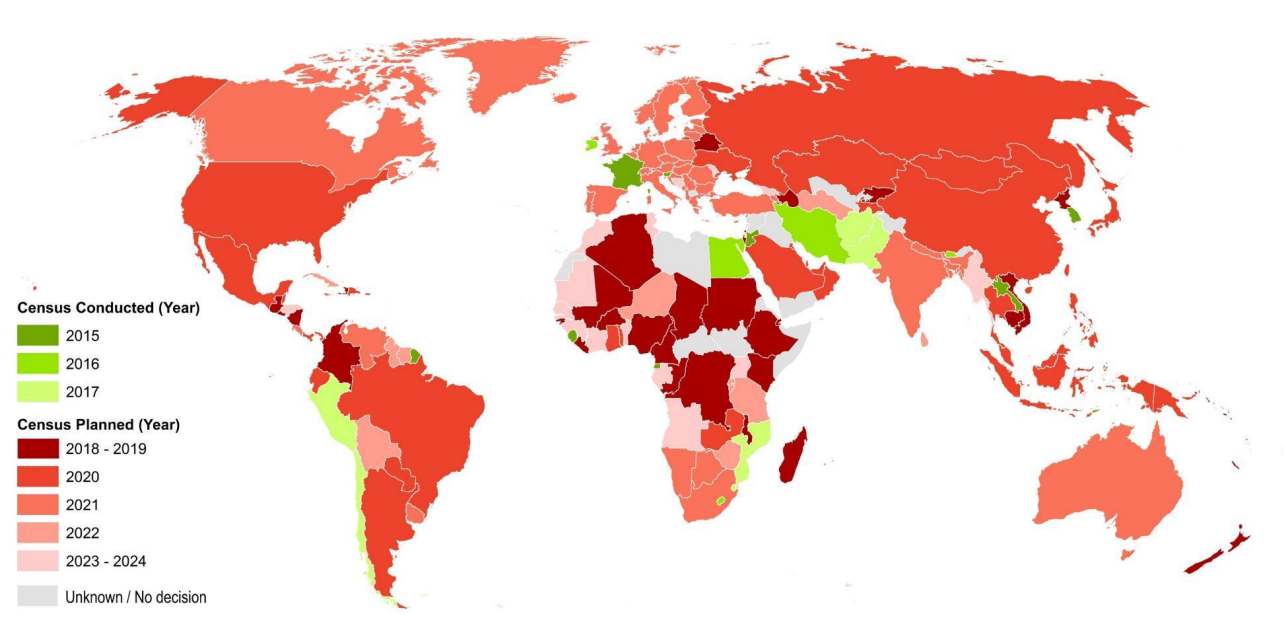
\includegraphics[scale=0.5]{images/most-recent-census-conducting-year-world-map.png}
    \caption{National dates for 2020 round of population census \cite{WorldMapOf2020RoundCensus}}
    \label{img:most-recent-census-conducting-year-world-map}
\end{figure}

With this information about the general population census conduct it is now possible to dive deeper in to the most popular census methods currently used around the world - self-reporting method, interview method and population registry analysis method with an additional alternative population census method offered and analysed.
\subsection{Traditional population census method overview}
\textbf{TO-DO: Write in detail about how the traditional population census works}

Conducting a traditional census typically requires a significant investment in resources. For instance, the 2020 U.S. Census cost around \$14 billion, covering personnel, technology, and data processing \cite{UsaCensusCost}. These costs often increase with the complexity and size of a country's population, as well as with efforts to ensure inclusivity and accurate counting, especially in remote or hard-to-reach areas.

\subsubsection{Self-reporting method}
\textbf{SHOULD THESE BE MERGED TOGETHER?}
\subsubsection{Interview method}
\subsection{Population registry analysis method overview}
\textbf{TO-DO: Write in detail about how the population registry analysis population census method works}
\subsection{Alternative population census method overview}

% Methodologies
\section{Population forecasting methodologies}
\textbf{TO-DO: General information about this chapter and methodologies used in this work}
\subsection{Preparation of the dataset}
\textbf{TO-DO: Write about the dataset used (satellite images + population census information)}
\subsection{Convolutional neural networks}
\textbf{TO-DO: Write about CNNs in general, their use cases}
\subsubsection{EfficientNet}
\textbf{TO-DO: Write in depth about the EfficientNet model and how does it stand out in terms of others}
\subsubsection{ResNet}
\textbf{TO-DO: Write in depth about the ResNet model and how does it stand out in terms of others}
\subsubsection{DenseNet}
\textbf{TO-DO: Write in depth about the DenseNet model and how does it stand out in terms of others}
\subsubsection{VGGNet}
\textbf{TO-DO: Write in depth about the VGGNet model and how does it stand out in terms of others}
\subsection{Results evaluation steps}
\textbf{TO-DO: Write about how the results will be analyzed and compared in order to find the best model for the bachelor's task}

% Implementation
\section{Population forecasting implementation}

% Results
\sectionnonum{Results}
Rezultatų skyriuje išdėstomi pagrindiniai darbo rezultatai: kažkas išanalizuota,
kažkas sukurta, kažkas įdiegta. Tarpinių žingsnių išdavos skirtos užtikrinti galutinio
rezultato kokybę neturi būti pateikiami šiame skyriuje. Kalbant informatikos termi-
nais, šiame skyriuje pateikiama darbo išvestis, kuri gali būti įvestimi kituose panašios
tematikos darbuose. Rezultatai pateikiami sunumeruotų (gali būti hierarchiniai) sąrašų
pavidalu. Darbo rezultatai turi atitikti darbo tikslą.

% Conclusions
\sectionnonum{Conclusions}
\begin{enumerate}[labelindent=0pt]
    \item Išvadų skyriuje daromi nagrinėtų problemų sprendimo metodų palyginimai, siūlomos
rekomendacijos, akcentuojamos naujovės.
    \item Išvados pateikiamos sunumeruoto (gali būti hierarchinis) sąrašo pavidalu.
    \item Darbo išvados turi atitikti darbo tikslą.
\end{enumerate}

% References
\printbibliography[heading=bibintoc]

% Abbreviations
% \sectionnonum{Sąvokų apibrėžimai}
\sectionnonum{Abbreviations}
Sąvokų apibrėžimai ir santrumpų sąrašas sudaromas tada, kai darbo tekste
vartojami specialūs paaiškinimo reikalaujantys terminai ir rečiau sutinkamos
santrumpos.

\end{document}